\section*{Exercise 5}
I have managed to implement the Random Midpoint Displacement Fractal in an unconventional way: The algorithm has been worked out in C\#. The C\# code performs the algorithm and exports the coordinates of the terrain to a .txt file, which can then be imported into Matlab and plotted. A simple example of the generated terrain can be found in the following image.\\

\begin{figure}[ht]
	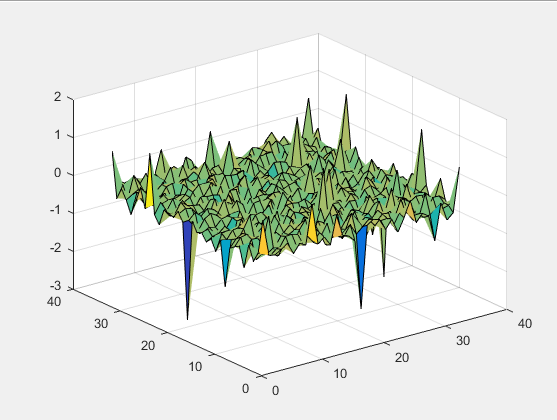
\includegraphics{images/surface}
	\caption{Surface plot of the Random Midpoint Displacement Fractal}
\end{figure}

I have included the C\# files in the project folder.